%%% Содержимое слайдов

% 1. Название, автор, руководитель.
% 2. Постановка задачи (актуальность)
% 3. способ (инструменты для) решения
% 4. результаты
% 5. анализ результатов
% 6. Заключение 

\frame[plain]{\titlepage} % Титульный слайд

%-------------------------------------------------------------------------------

\section{Постановка задачи}

\begin{frame}
\frametitle{\insertsection}

% \textbf{Задачи:}
% \begin{itemize}    
%     \item палетки с любыми параметрами (без ограничений времени)
%     \item оценка возможности решения обратной задачи БКЗ в реальном времени
% \end{itemize}

\textbf{Акутальность:}
\begin{itemize}
\item Решение полных постановок задач весьма ресурсоемко
\item Задача разработки метода решения прямой задачи БКЗ
\item Решение математической постановки прямой задачи БКЗ неэффективно уже имеющимися средствами
\end{itemize}
\bigskip

\textbf{Краевая задачв:}
\begin{alignat}{2}
\nabla \cdot (\nabla u(\bm x) / \rho(\bm x)) &= -I \delta(\bm x),\qquad && \bm x \in \varOmega, \label{eq:poisson}\\
u(\bm x) &= 0, && \bm x \in \partial \varOmega. \label{eq:dirichet}
\end{alignat}
\end{frame}

\begin{frame}
\frametitle{\insertsection}

\begin{minipage}[t]{0.47\linewidth}
    \textbf{Модель 1}
    \center{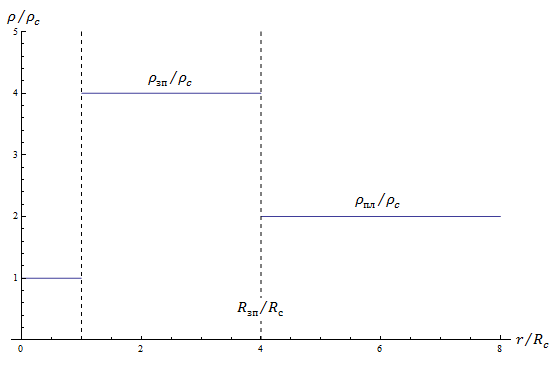
\includegraphics[width=1\linewidth]{rho_model_1.png}}
\end{minipage}
\hfill
\begin{minipage}[t]{0.47\linewidth}
    \textbf{Модель 2}
    \center{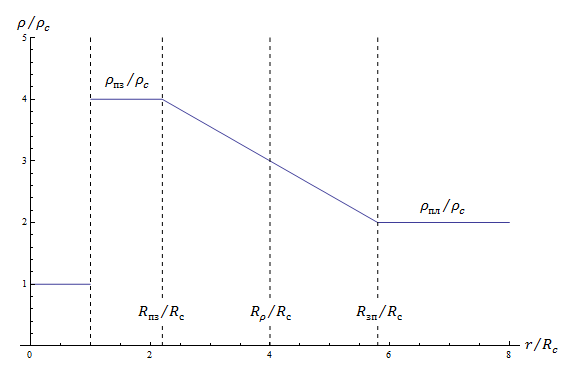
\includegraphics[width=1\linewidth]{rho_model_2.png}}
\end{minipage}
\end{frame}
%-------------------------------------------------------------------------------

\section{Способ решения}

\begin{frame}
\frametitle{\insertsection}

\textbf{Инструменты:}
\begin{itemize}
    \item Язык программирования Python
    \item Вычислительная платформа FEniCS
    \item Модуль triangle для триангуляции Делоне
    \item Компьютер: ОС Ubuntu 18.04 LTS, процессор Intel Pentium 4415U 2.30 ГГц
\end{itemize}
\end{frame}

Построение расчетной сетки с заданием узлов и графа для триангуляции расчетной области с помощью библиотеки triangle.

\begin{frame}
\frametitle{\insertsection}

Расчетная сетка:
\begin{itemize}
\item расположения узлов на расчетной области
\begin{itemize}
  \item лучи, на которых лежат узлы
  \item расположения узлов на лучах
\end{itemize}
\item варианты графов
\item расположения узлов на границах зон
\item дополнительные узлы при триангуляции
\end{itemize}

Решение методом конечных элементов на расчетной сетке:
\begin{itemize}
    \item различные степени полиномов
\end{itemize}
\end{frame}

\begin{frame}
\frametitle{\insertsection}

Оптимальная расчетная схема:
\begin{itemize}
    \item лучи, на которых лежат узлы
    \item узлы на лучах, равноотстоящие в логарифмическом масштабе;
    \item вторая степень полинома
    \item узлы на пересечениях границ зон с лучами и с концентрическими окружностями
\end{itemize}
\end{frame}

%-------------------------------------------------------------------------------

\section{Результаты}

\begin{frame}
\frametitle{\insertsection}

\vspace{-0.5cm}
\begin{minipage}[t]{0.47\linewidth}
    \textbf{Модель 1}
    \center{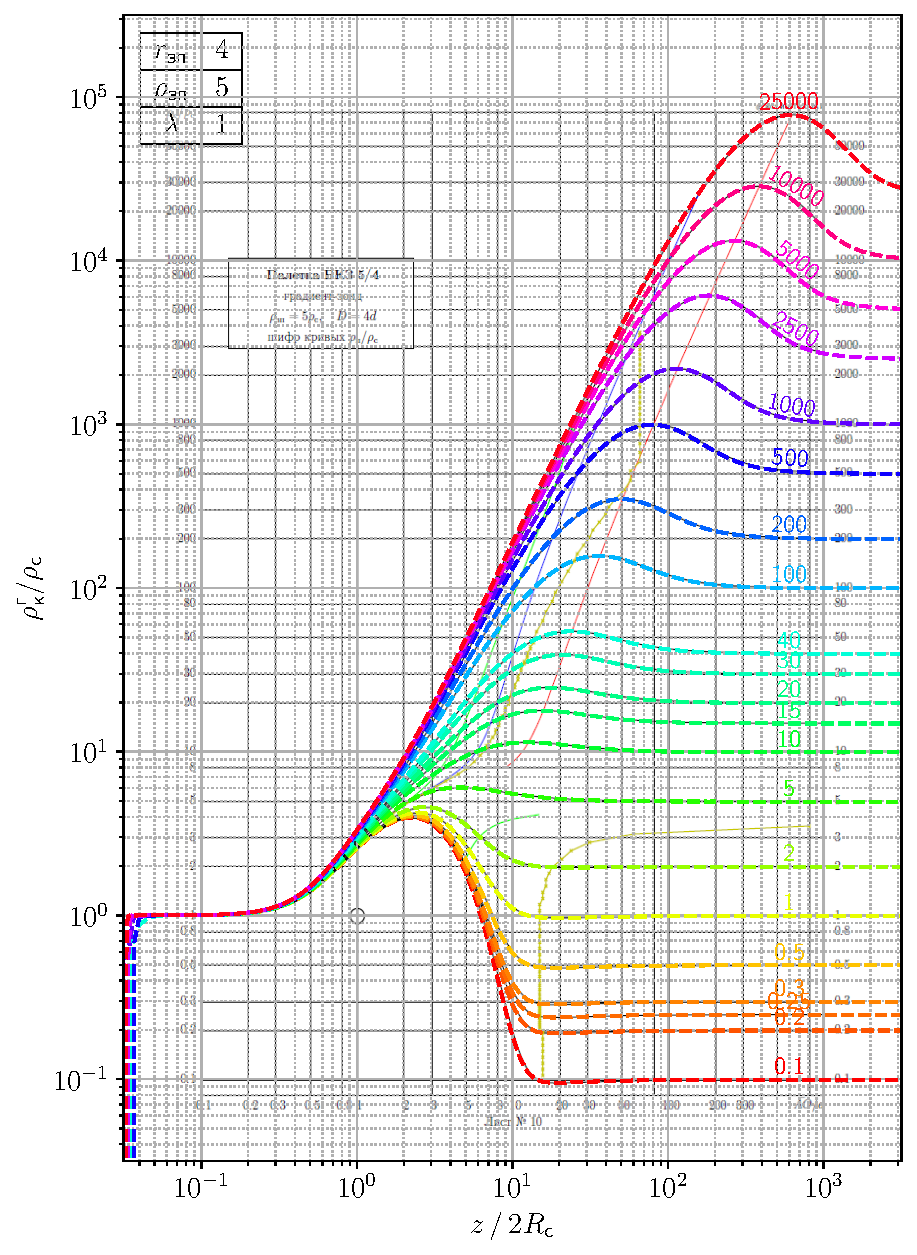
\includegraphics[width=1\linewidth]{plot_1_compare}}
\end{minipage}
\hfill
\begin{minipage}[t]{0.47\linewidth}
    \textbf{Модель 2}
    \center{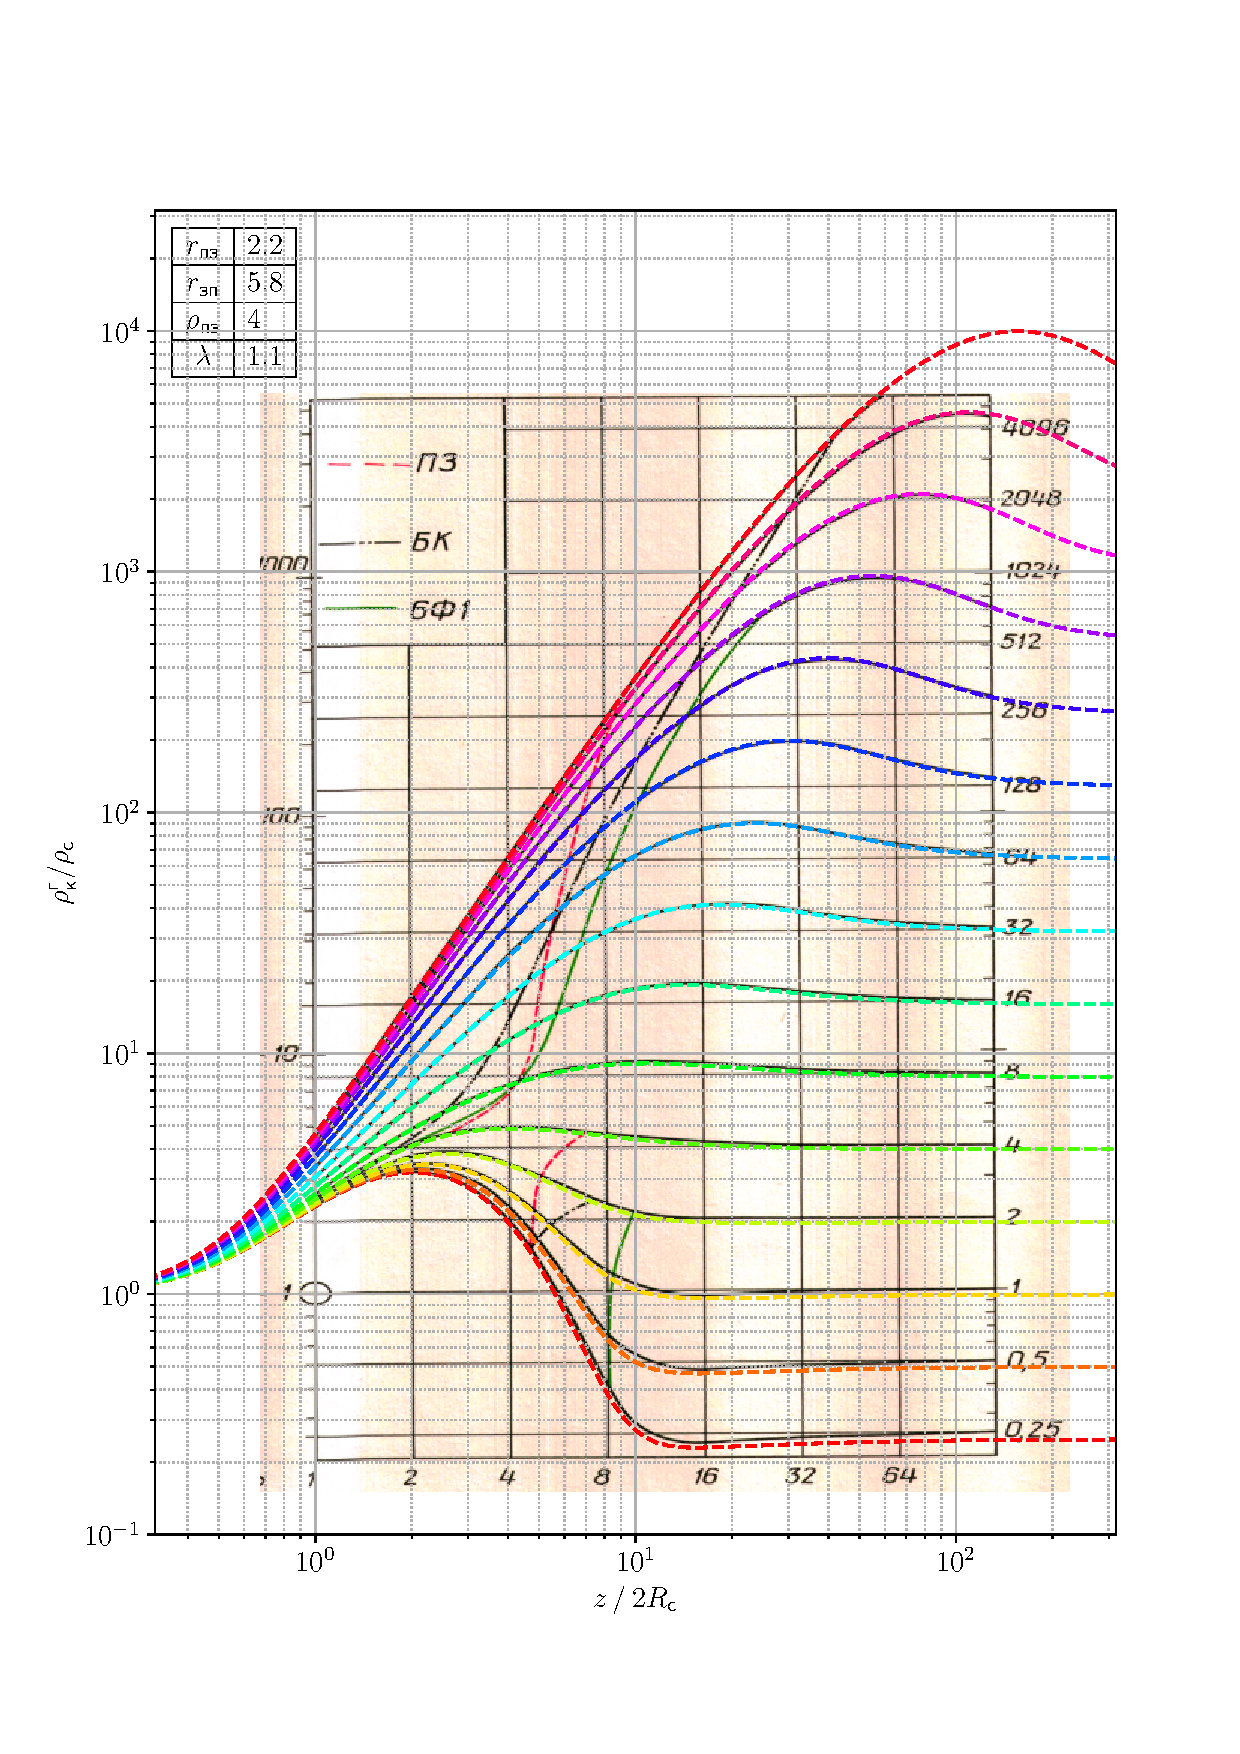
\includegraphics[width=1\linewidth]{plot_2_compare}}
\end{minipage}

\end{frame}

%-------------------------------------------------------------------------------

\section{Анализ результатов}

\begin{frame}
\frametitle{\insertsection}

\textbf{Модель 1:}
\begin{itemize}
    \item Время вычисления расчетной палетки 17.421 с
    \item 4669 узлов расчетной сетки
\end{itemize}
\bigskip

\textbf{Модель 2:}
\begin{itemize}
    \item Время вычисления расчетной палетки 17.839 с
    \item 4813 узлов расчетной сетки
\end{itemize}
\bigskip

\textbf{Критерии точности решения}:
\begin{itemize}
    \item гладкость решения
    \item сравнение "на глаз" решения с известным
\end{itemize}
\end{frame}

%-------------------------------------------------------------------------------

\section{Заключение}

\begin{frame}
\frametitle{\insertsection}

\begin{itemize}
    \item Освоены пакеты программ для параллельных вычислений
    \item Проведены расчеты и сопоставление с известными результатами в литературе
    \item Показана применимость метода решения прямой задачи БКЗ
\end{itemize}
\end{frame}

%-------------------------------------------------------------------------------

\section{Конец}

\begin{frame}
\centering
\vfill
\textcolor{Blue}{\Large Спасибо за внимание!}
\vfill
\end{frame}